
\section{The Full Model}
After we did one more experiment that is explained in the appendix
 I could could examine the measured values and made some observations that are
  described in this section. Based on those observations I built the full model
   that will be the basis of a mean value analysis shown further in the document.

\subsection{Definitions}
blablab

\subsection{Observations}
This is a table (table \ref{table:measuredData}) measured throughout the
 and a footnote \footnote{Described in the appendix \ref{sec:client_scale_out}} 
 
\begin{table}[h!]
 \centering
 \begin{tabular}{| r| rrrr | rr | r |}
    \hline \textbf{$N$} & \textbf{$R_{puts}$} & \textbf{$R_{retrieves}$} & \textbf{$R_{meas}$} & \textbf{$X_{meas}$} & \textbf{$X_{calc}$} & \textbf{$R_{calc}$}  & \textbf{$Z_{calc}$} \\
    \hline 32  & 69  & 112 & 181 & 176.5 & 176.8 & 181 & 0 \\
    \hline 64  & 72  & 113 & 185 & 344.7 & 345.9 & 186 & 1 \\
    \hline 96  & 81  & 115 & 196 & 486.4 & 489.8 & 197 & 1 \\
    \hline 128 & 98  & 119 & 217 & 586.8 & 589.9 & 218 & 1 \\
    \hline 160 & 124 & 130 & 254 & 628.3 & 629.9 & 255 & 1 \\
    \hline 192 & 161 & 156 & 317 & 603.9 & 605.7 & 318 & 1 \\
    \hline 224 & 213 & 204 & 417 & 536.4 & 537.2 & 418 & 1 \\
    \hline 256 & 251 & 230 & 481 & 531.2 & 532.2 & 482 & 1 \\ 
    \hline
 \end{tabular}
\caption{Measured (on client side) and calculated data of the whole system.}
\label{table:measuredData}
\end{table}


\subsection{The Model}
and a figure \ref{fig:full_model}.  fancy foobar

\begin{figure}[h!]
\centering
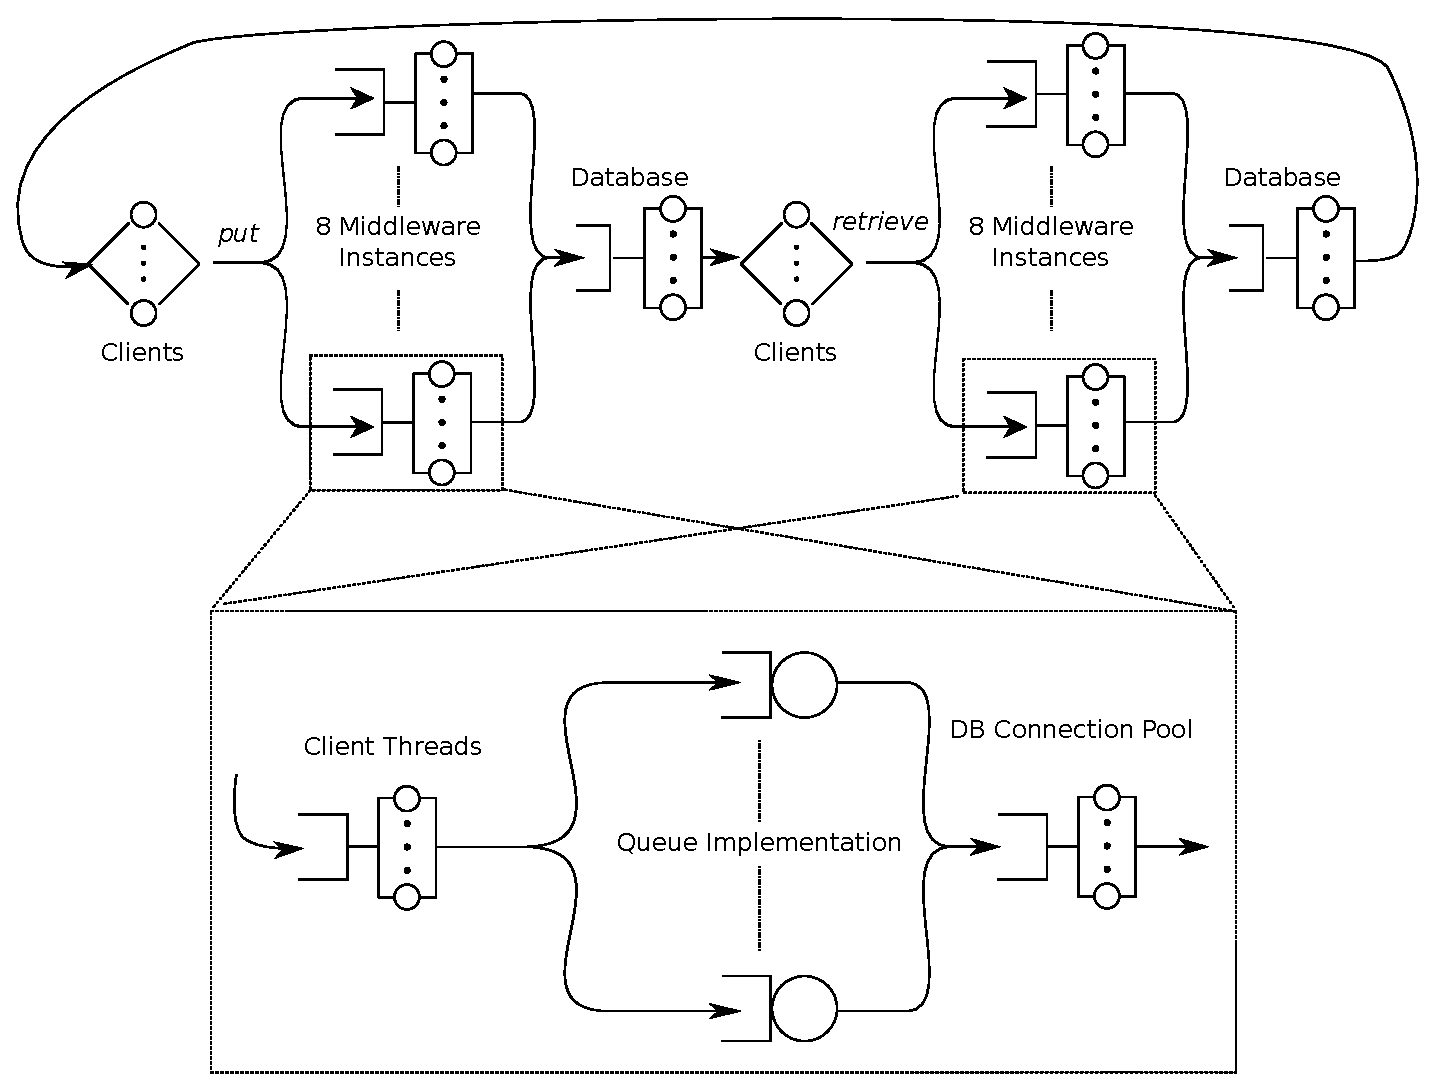
\includegraphics[width=1\textwidth]{figures/full_model.eps}
\caption{Full model of the system.}
\label{fig:full_model}
\end{figure}

\newpage

citation\cite{lz77}. 

some math

\[\mu(n) =
\left\{
	\begin{array}{ll}
		n/S  & \mbox{if } n=1,2,...,m-1 \\
		m/S & \mbox{if } n=m,m+1,...,\infty
	\end{array}
\right.
 \]


